\chapter{Crash Test/Consistency Report}
\section{Crash Test/Consistency Report}
\begin{enumerate}
    \item Courses \\ \\ 
    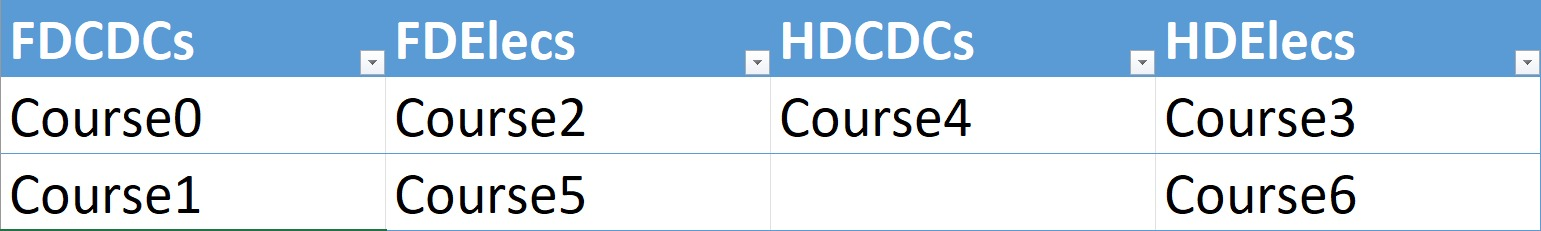
\includegraphics[width=12cm, height=2cm]{Courses4}
    \item Professors \\ \\ 
    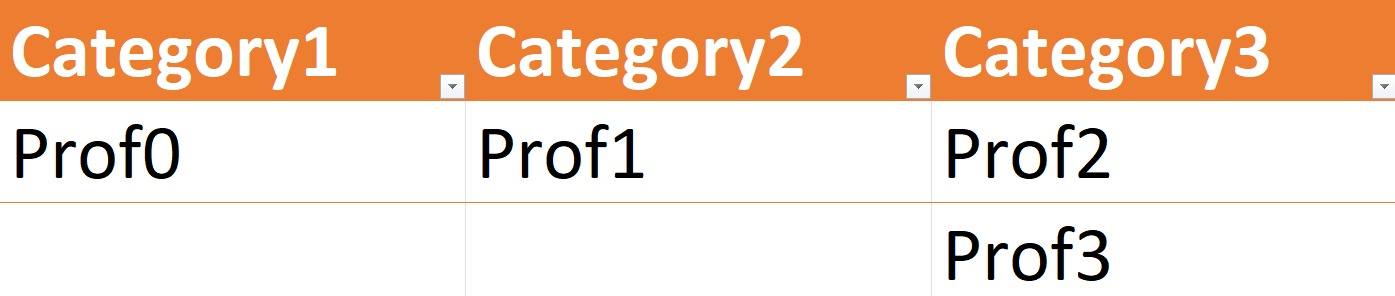
\includegraphics[width=12cm, height=2cm]{images/Professors4.jpeg}
    \item Preferences \\ \\
    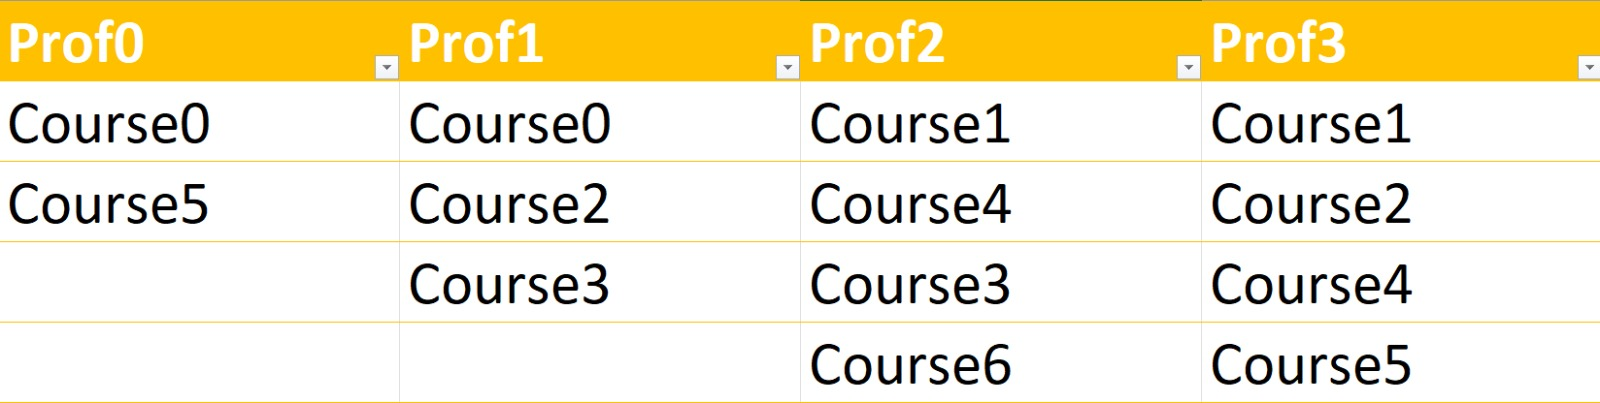
\includegraphics[width=12cm, height=2cm]{images/Preferences4.jpeg}
    \item
    \begin{figure}[h]
    \centering
    \caption{Bipartite Matching: Upper nodes are units of Professors while lower nodes are units of Courses.}
    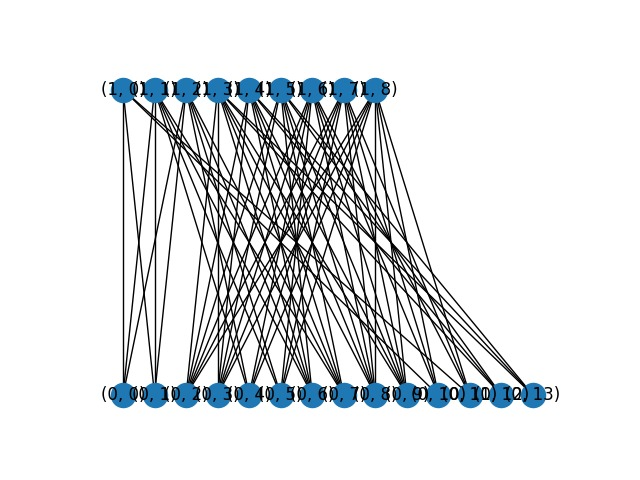
\includegraphics[width=0.5\textwidth]{images/Graph4.jpeg}
    \end{figure}\\
    Output \\ \\
    Number of satisfactory matchings: 15 \\ \\
52 : (('Prof0', 'Course0', 1), ('Prof1', 'Course0', 1), ('Prof1', 'Course2', 1), ('Prof2', 'Course4', 2), ('Prof2', 'Course1', 1), ('Prof3', 'Course2', 1), ('Prof3', 'Course1', 1))\\ \\
52 : (('Prof0', 'Course0', 1), ('Prof1', 'Course2', 1), ('Prof1', 'Course0', 1), ('Prof2', 'Course4', 2), ('Prof3', 'Course2', 1), ('Prof3', 'Course1', 2))\\ \\
51 : (('Prof0', 'Course0', 1), ('Prof1', 'Course2', 1), ('Prof1', 'Course0', 1), ('Prof2', 'Course1', 2), ('Prof2', 'Course4', 1), ('Prof3', 'Course2', 1), ('Prof3', 'Course4', 1))\\ \\
51 : (('Prof0', 'Course0', 1), ('Prof1', 'Course2', 1), ('Prof1', 'Course0', 1), ('Prof2', 'Course4', 1), ('Prof2', 'Course1', 1), ('Prof3', 'Course2', 1), ('Prof3', 'Course4', 1), ('Prof3', 'Course1', 1))\\ \\
50 : (('Prof0', 'Course5', 1), ('Prof1', 'Course0', 2), ('Prof2', 'Course4', 2), ('Prof2', 'Course1', 1), ('Prof3', 'Course5', 1), ('Prof3', 'Course1', 1))\\ \\
50 : (('Prof0', 'Course5', 1), ('Prof1', 'Course0', 2), ('Prof2', 'Course4', 2), ('Prof3', 'Course5', 1), ('Prof3', 'Course1', 2))\\ \\
50 : (('Prof0', 'Course0', 1), ('Prof1', 'Course0', 1), ('Prof1', 'Course3', 1), ('Prof2', 'Course4', 2), ('Prof2', 'Course3', 1), ('Prof3', 'Course1', 2))\\ \\
50 : (('Prof0', 'Course0', 1), ('Prof1', 'Course2', 1), ('Prof1', 'Course0', 1), ('Prof2', 'Course1', 2), ('Prof3', 'Course2', 1), ('Prof3', 'Course4', 2))\\ \\
49 : (('Prof0', 'Course5', 1), ('Prof1', 'Course0', 2), ('Prof2', 'Course4', 1), ('Prof2', 'Course1', 2), ('Prof3', 'Course5', 1), ('Prof3', 'Course4', 1))\\ \\
49 : (('Prof0', 'Course5', 1), ('Prof1', 'Course0', 2), ('Prof2', 'Course4', 1), ('Prof2', 'Course1', 1), ('Prof3', 'Course5', 1), ('Prof3', 'Course4', 1), ('Prof3', 'Course1', 1))\\ \\
49 : (('Prof0', 'Course0', 1), ('Prof1', 'Course0', 1), ('Prof1', 'Course3', 1), ('Prof2', 'Course4', 1), ('Prof2', 'Course1', 1), ('Prof2', 'Course3', 1), ('Prof3', 'Course4', 1), ('Prof3', 'Course1', 1))\\ \\
49 : (('Prof0', 'Course0', 1), ('Prof1', 'Course0', 1), ('Prof1', 'Course3', 1), ('Prof2', 'Course4', 1), ('Prof2', 'Course3', 1), ('Prof3', 'Course1', 2), ('Prof3', 'Course4', 1))\\ \\
48 : (('Prof0', 'Course0', 1), ('Prof1', 'Course0', 1), ('Prof1', 'Course3', 1), ('Prof2', 'Course1', 2), ('Prof2', 'Course3', 1), ('Prof3', 'Course4', 2))\\ \\
48 : (('Prof0', 'Course0', 1), ('Prof1', 'Course0', 1), ('Prof1', 'Course3', 1), ('Prof2', 'Course1', 1), ('Prof2', 'Course3', 1), ('Prof3', 'Course4', 2), ('Prof3', 'Course1', 1))\\ \\
48 : (('Prof0', 'Course5', 1), ('Prof1', 'Course0', 2), ('Prof2', 'Course1', 2), ('Prof3', 'Course5', 1), ('Prof3', 'Course4', 2))\\ \\
Time: 1690.72 seconds (28.18 mins)

\paragraph{} The code is uniform in writing and consistent in its output. It may take time to run as time complexity is high, but will give all possible desirable maximum matchings without crashing. For example, the test case above took 28.18 minutes, but successfully gave us an output.
\paragraph{} If a CDC is not a part of the preference order of any professor, the code lets us know without crashing. If there are no satisfactory matchings, then it still does not crash and informs us of the same.

\end{enumerate}